\documentclass[11pt]{article}
\usepackage{geometry}
\usepackage{amsmath}
\usepackage{amssymb}
\usepackage{enumitem}
\usepackage{fancyhdr}
\usepackage{graphicx}
\usepackage{lastpage}
\usepackage{parskip}
\usepackage{siunitx}
\usepackage{listings} % to include code

\newif\ifclearpage

\newcommand{\name}{}
\newcommand{\class}{Math 155, Fall 2018}
\newcommand{\assignment}{Problem Set 7}
\newcommand{\duedate}{Due Thursday, November 15}
\newcommand{\rpm}{\sbox0{$1$}\sbox2{$\scriptstyle\pm$}
  \raise\dimexpr(\ht0-\ht2)/2\relax\box2 }

\clearpagetrue

\newcommand{\problem}[1]{\section*{#1}}
\newcommand{\solution}{\hrulefill}
\newcommand{\maybeclearpage}{\ifclearpage\clearpage\fi}

\renewcommand{\vec}[1]{\mathbf{#1}}

\geometry{margin=1in}

\fancypagestyle{primary}{
  \fancyhf{}
  \lhead{\name}
  \chead{\assignment}
  \rhead{\class}
  \lfoot{\duedate}
  \rfoot{\thepage{} of \pageref{LastPage}}}

\pagestyle{primary}

\setlist[enumerate]{label=(\alph*)}

\sisetup{per-mode=symbol}

\begin{document}

\problem{Chapter 6, Problem 4}
Add new entries to Exhibit 6.11 on page 111, for the following values:
\begin{enumerate}
\item $\phi = \rpm 0.99$.
\item $\phi = \rpm 0.5$.
\item $\phi = \rpm 0.1$.
\end{enumerate}

\solution


\maybeclearpage
\problem{Chapter 6, Problem 13}
A stationary time series of length 121 produced sample partial autocorrelation of $\hat{\phi}_{11} = 0.8$, $\hat{\phi}_{22} = -0.6$, $\hat{\phi}_{33} = 0.08$, and $\hat{\phi}_{44} = 0.00$. Based on this information alone, what model would we tentatively specify for the series?

\solution


\maybeclearpage
\problem{Chapter 6, Problem 15}
The sample ACF for a series and its first difference are given in the following table. Here $n = 100$.

\begin{center}[]
\begin{tabular}{lllllll}
 \textbf{lag} & \textbf{1} & \textbf{2} & \textbf{3} & \textbf{4} & \textbf{5} & \textbf{6} \\
 ACF for $Y_t$ & 0.97 & 0.97 & 0.93 & 0.85 & 0.80 & 0.71 \\
 ACF for $\nabla Y_t$ & -0.42 & 0.18 & -0.02 & 0.07 & -0.10 & -0.09
\end{tabular}
\end{center}

Based on this information alone, which ARIMA model(s) would we consider for the series?

\solution

\maybeclearpage
\problem{Chapter 6, Problem 17}
Consider an AR(1) series of length 100 with $\phi = 0.7$.
\begin{enumerate}
\item Would you be surprised if $r_1 = 0.6$?
\item Would $r_{10} = -0.15$ be unusual?
\end{enumerate}

\solution


\maybeclearpage
\problem{Chapter 6, Problem 19}
The time plots of two series are shown below.
\begin{enumerate}
	\item For each of the series, describe $r_1$ using the terms strongly positive, moderately positive, near zero, moderately negative, or strongly negative. Do you need to know the scale of measurement for the series to answer this?
	\item Repeat part (a) for $r_2$.
\end{enumerate}

\centerline{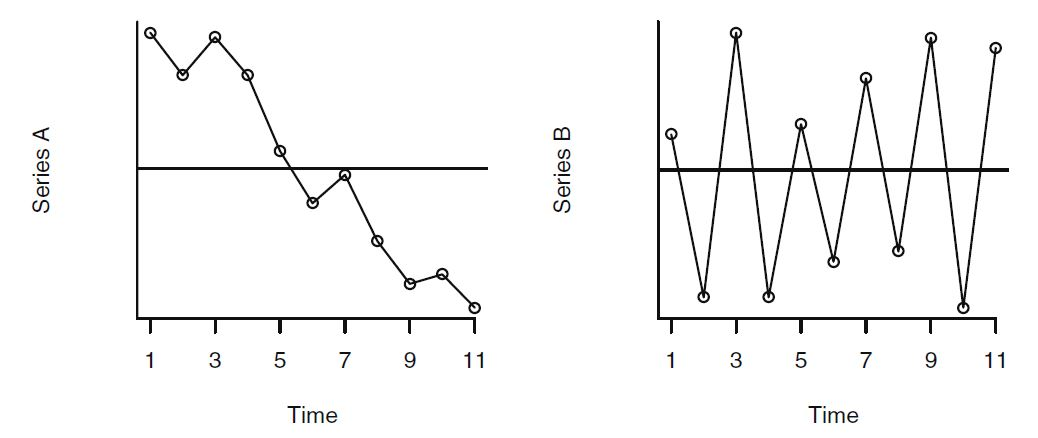
\includegraphics{graphs.jpg}}

\solution


\maybeclearpage

\end{document}